\section{Một số khái niệm}
\subsection{Chuẩn hóa tập mẫu}
\begin{frame}
\frametitle{Chuẩn hóa tập mẫu}
	\begin{itemize}
    \item Chuẩn hóa là một phương pháp tiền xử lý thiết yếu, đặc biệt là trong trường hợp các biến quan sát được đo lường bằng những đơn vị hoặc những thang đo khác nhau (VD: mét, kilogram hay đơn vị tiền tệ). 
    \item Sự khác biệt lớn giữa phạm vi các khoảng giá trị của các biến độc lập có thể tạo ra sự sai lệch trong phân tích để đưa ra một mô hình chính xác. 
    \item VD: Giả sử $z_1$ là biến dự đoán thể hiện chiều cao của một người, vậy thì $z_1 \in [0;2]$ với đơn vị mét. Giả sử $z_2$ là biến dự đoán thể hiện mức chi tiêu của một người (tính theo VNĐ), ta có thể có $z_2 \in [0;10 000 000 000]$. Trong trường hợp hai biến "chiều cao" và "chi tiêu" như trên, "chi tiêu" sẽ có tác động lớn hơn đối với đầu ra (biến phản hồi), nhưng như vậy ta không khẳng định được rằng biến đó có ý nghĩa quan trọng hơn về mặt thống kê. 
\end{itemize}
\end{frame}
%%=====================================
\begin{frame}
\frametitle{Chuẩn hóa tập mẫu}
	\begin{itemize}
	\item Để chuẩn hóa dữ liệu, ta đặt:
   \[
   z^* = \dfrac{z- \mu}{s}
   \]
   Trong đó:
   \begin{itemize}
       \item $z$ là giá trị quan sát
       \item $\mu$ là giá trị trung bình mẫu
       \item $s$ là độ lệch chuẩn
   \end{itemize}
   \item Tác dụng của việc chuẩn hóa dữ liệu:
   \begin{itemize}
       \item Đưa các biến về cùng thang đo.
       \item Tăng độ chính xác và ổn định của mô hình thống kê, tránh việc biến có giá trị lớn chi phối kết quả.
       \item Khi áp dụng công thức này với toàn bộ dữ liệu $Z$, ta sẽ nhận được mẫu $Z^*$ mới có $\mu = 0$ và $s=1$.
   \end{itemize}
	\end{itemize}
\end{frame}
%%=====================================
\subsection{Outlier}
\begin{frame}
\frametitle{Outlier}
	\begin{block}{Định nghĩa}
    \textbf{Outlier} là điểm dữ liệu bất thường, nghĩa là quan sát tại điểm đó khác biệt so với phần còn lại của bộ dữ liệu mà ta thu thập được. 
    \end{block}
    \begin{figure}
        \centering
        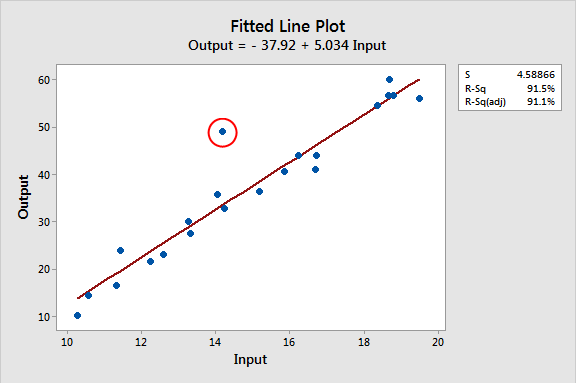
\includegraphics[width=0.55\linewidth]{images/Hình minh họa cho Outlier.png}
        \caption{Hình minh họa cho Outlier}
    \end{figure}
\end{frame}
%%=====================================
\begin{frame}
\frametitle{Sự tác động của Outlier đến mô hình hồi quy}
	\begin{figure}
	    \centering
	    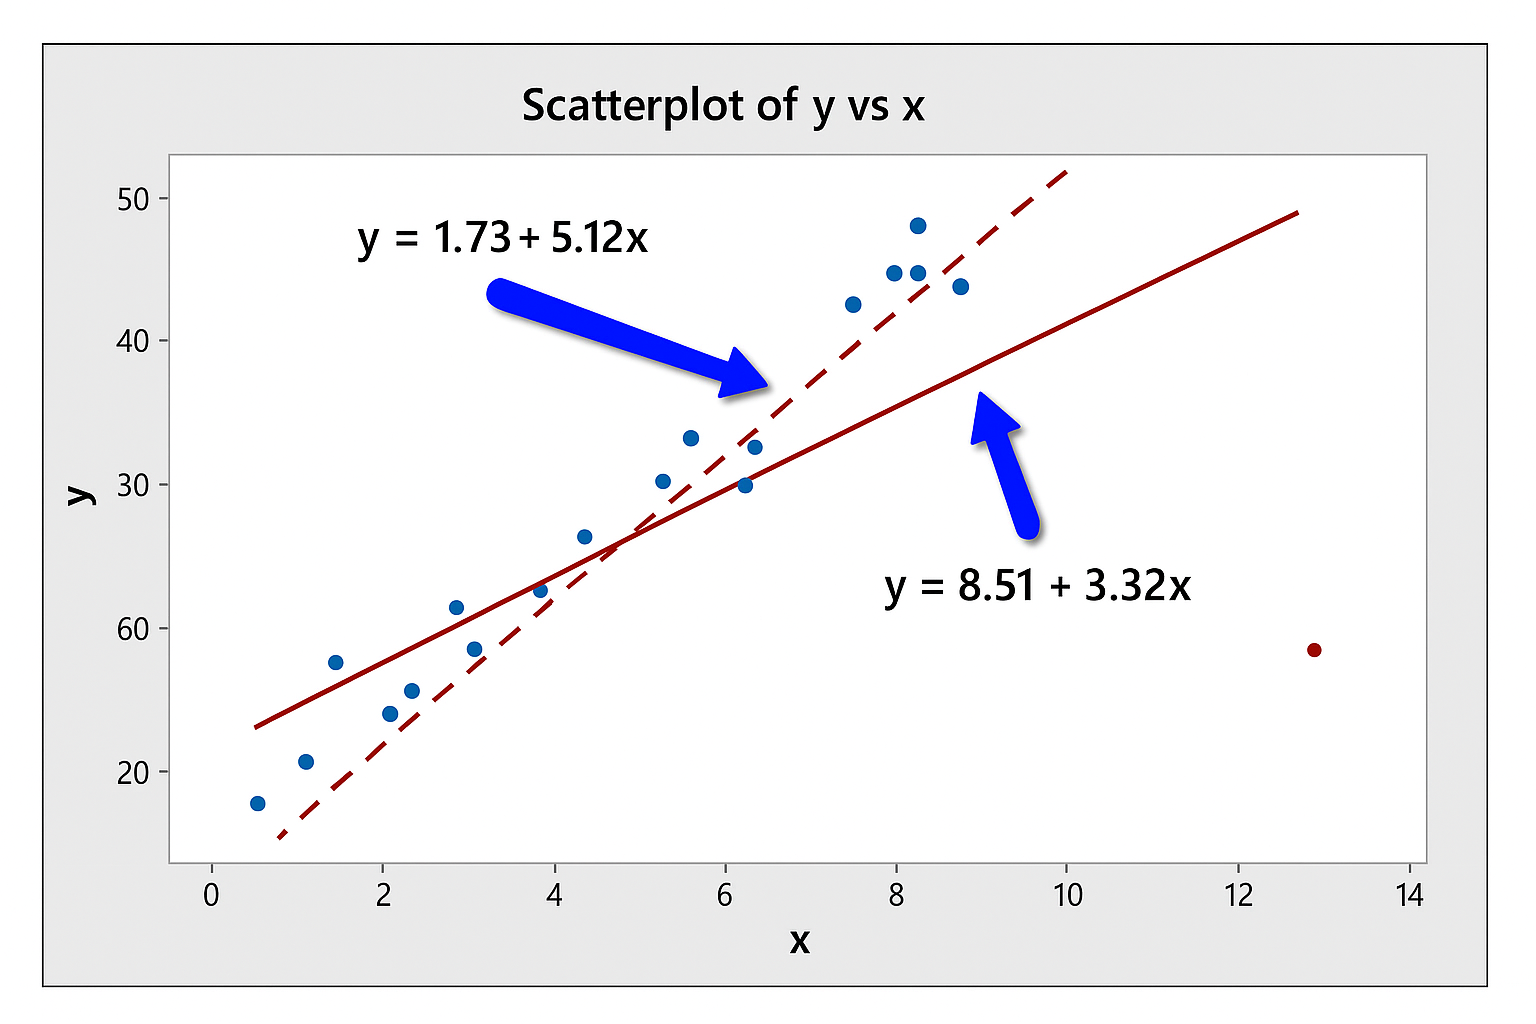
\includegraphics[width=0.6\linewidth]{images/Sự tác động của Outlier đến mô hình.png}
	    \caption{Sự tác động của Outlier đến mô hình}
	\end{figure}
    \begin{itemize}
        \item Đường nét liền thể hiện mô hình hồi quy tuyến tính khi giữ lại Outlier.
        \item Đường nét đứt thể hiện mô hình hồi quy tuyến tính khi đã loại bỏ Outlier.
    \end{itemize}
\end{frame}
\subsection{Độ đo Leverage}
\begin{frame}
\frametitle{Độ đo Leverage}
	\begin{itemize}
    \begin{block}{Định nghĩa}
    \textbf{Leverage} là độ đo khoảng cách giữa một điểm dữ liệu và phần còn lại của bộ dữ liệu dựa trên miền giá trị của bộ dữ liệu, được xác định bởi công thức:
    $$ h_{k j}=\frac{1}{n}+\frac{\left(z_{kj}-\overline{z}\right)^{2}}{\sum_{j=1}^{n}\left(z_{kj}-\overline{z}\right)^{2}}$$
    \end{block}
    \item Những điểm nằm xa so với bộ dữ liệu gọi là những điểm high leverage, ngược thì gọi là lower leverage.
    \item \textbf{Kết luận:} Ta thấy $h_{kj}$ luôn nằm giữa 1/n và 1. Hơn nữa, leverage trung bình cho các quan sát luôn bằng (p+1)/n, p là biến số dự đoán. Do vậy, nếu một quan sát mà có độ đo leverage quá lớn so với (p+1)/n ta có thể nghi ngờ là một điểm high leverage.
\end{itemize}
\end{frame}
%%=====================================
\begin{frame}
\frametitle{Nhận xét}
\begin{itemize}
   \item Càng có nhiều điểm dữ liệu nằm gần nhau thì sức ảnh hưởng hay độ lớn của điểm high leverage càng giảm.
   \item Các điểm high leverage có tác động rất lớn đến mô hình, điểm nào có giá trị của biến dự đoán nằm càng xa khỏi bộ dữ liệu thì tác động càng lớn.
   \item Những điểm $h_{kj} > 3*\overline{h}$ thì được coi là những outlier, với $\overline{h} = \dfrac{1}{n}\sum_{j=1}^n{h_{kj}}$
\end{itemize}
\end{frame}
%%=====================================
\begin{frame}
\frametitle{Ví dụ}

Để nghiên cứu sự phụ thuộc giữa điểm thi cuối kỳ $Y$ (tính theo thang 10) và số giờ tự học mỗi tuần $Z_1$, số giờ ngủ trung bình mỗi đêm $Z_2$ (đơn vị giờ), người ta điều tra ngẫu nhiên 12 sinh viên đại học của một trường, thu được bảng số liệu sau:

\resizebox{\textwidth}{!}{%
\begin{tabular}{|c|c|c|}
\hline 
$Y$ (Điểm thi cuối kỳ) & $Z_1$ (Số giờ tự học mỗi tuần) & $Z_2$ (Số giờ ngủ trung bình mỗi đêm) \\
\hline 
5.8 & 6.5 & 6.5 \\
6.5 & 7.0 & 6.0 \\
7.0 & 6.5 & 7.0 \\
7.5 & 8.0 & 6.5 \\
8.0 & 9.0 & 7.2 \\
8.2 & 10.0 & 6.8 \\
7.8 & 8.6 & 7.5 \\
8.8 & 11.0 & 7.0 \\
9.0 & 12.0 & 6.7 \\
6.0 & 6.0 & 6.0 \\
8.3 & 9.5 & 7.8 \\
9.2 & 2.0 & 5.5 \\
\hline
\end{tabular}%
}

\end{frame}

%%=====================================
\begin{frame}
\frametitle{Ví dụ}

Ta có bảng sau:

\resizebox{\textwidth}{!}{%
\begin{tabular}{|c|ccc|c|ccc|}
\hline 
$j$ & $z_1$ & $h_{1j}$ & $h_{1 j} > 3*\frac{1}{n}\sum_{j=1}^{n}{h_{1 j}}$ 
& $j$ & $z_2$ & $h_{2j}$ & $h_{2 j} > 3*\frac{1}{n}\sum_{j=1}^{n}{h_{2 j}}$ \\
\hline
1 & 6.5 & 0.1125 & 0 & 1 & 6.5 & 0.0924 & 0 \\
2 & 7.0 & 0.0964 & 0 & 2 & 6.0 & 0.1881 & 0 \\
3 & 6.5 & 0.1125 & 0 & 3 & 7.0 & 0.1011 & 0 \\
4 & 8.0 & 0.0833 & 0 & 4 & 6.5 & 0.0924 & 0 \\
5 & 9.0 & 0.0959 & 0 & 5 & 7.2 & 0.1338 & 0 \\
6 & 10.0 & 0.1341 & 0 & 6 & 6.8 & 0.0851 & 0 \\
7 & 8.6 & 0.0878 & 0 & 7 & 7.5 & 0.2142 & 0 \\
8 & 11.0 & 0.1979 & 0 & 8 & 7.0 & 0.1011 & 0 \\
9 & 12.0 & 0.2873 & 0 & 9 & 6.7 & 0.0833 & 0 \\
10 & 6.0 & 0.1350 & 0 & 10 & 6.0 & 0.1881 & 0 \\
11 & 9.5 & 0.1118 & 0 & 11 & 7.8 & 0.3322 & 0 \\
12 & 2.0 & 0.5455 & 1 & 12 & 5.5 & 4.7122 & 1 \\
\hline
\end{tabular}%
}

\vspace{0.5em}
Trong bộ dữ liệu ở ví dụ 6.1, quan sát thứ 12 ($Y=9.2$, $z_1 = 2.0$, $z_2 = 5.5$) là một \textbf{outlier} vì điểm này có kết quả thi rất cao mặc dù thời gian học và ngủ thấp, trái ngược với xu hướng chung.
\end{frame}

%%======================
%%=====================================
\subsection{Quy tắc 1.5IQR}
\begin{frame}
\frametitle{Quy tắc 1.5IQR}
\begin{itemize}
    \item Bất kì tập dữ liệu nào cũng có thể mô tả bằng năm giá trị đặc trưng, năm giá trị này cung cấp thông tin cần thiết để định vị outlier bao gồm (lần lượt theo thứ tự tăng dần).
    \begin{itemize}
        \item Giá trị nhỏ nhất hoặc thấp nhất của tập dữ liệu.
        \item Tứ phân vị thứ nhất $Q_1$: Phân vị mức 25\%.
        \item Tứ phân vị thứ hai $Q_2$: Phân vị mức 50\%.
        \item Tứ phân vị thứ ba $Q_3$: Phân vị mức 75\%.
        \item Giá trị lớn nhất hoặc cao nhất của tập dữ liệu.
    \end{itemize}
    \item \textbf{Khoảng cách tứ phân vị} là giá trị
    \[
    IQR = Q_3 - Q_1
    \]
    Khi đó nếu $x \notin \left[Q_1 - 1.5IQR, Q_3 + 1.5IQR\right]$ thì $x$ sẽ được coi là một điểm outlier.
\end{itemize}
\end{frame}
%%=====================================
%%=====================================
\begin{frame}
\frametitle{Ví dụ}
	    Một hệ thống ghi lại tốc độ (đơn vị: km/h) của 25 xe qua trạm như sau: 
        \begin{center}
            \begin{tabular}{|c|c|c|c|c|c|c|c|c|c|c|c|c|}
	\hline 
	20 & 41 & 41 & 80 & 40 & 52 & 52 & 52 & 60 & 55 & 60 & 60 & 62 \\ \hline
60 & 55 & 60 & 55 & 92 & 70 & 35 & 40 & 30 & 30 & 80 & 25 &  \\ \hline
\end{tabular}
        \end{center}
        Tìm các số liệu bất thường (nếu có) trong mẫu số liệu trên.
\end{frame}
%%=====================================
\begin{frame}
\frametitle{Ví dụ}
\begin{itemize}
	\item Sắp xếp dữ liệu theo thứ tự tăng dần: 20, 25, 30, 30, 35, 40, 40, 41, 41, 52, 52, 52, 55, 55,  60, 60, 60, 60, 60, 62, 70, 80, 80, 92.
    \item $Q_1$ là trung bình cộng giá trị thứ 6 và 7 nên $Q_1 = \dfrac{40 + 40}{2} = 40$.
    \item $Q_3$ là trung bình cộng giá trị thứ 19 và 20 nên $Q_3 = \dfrac{60 + 60}{2} = 60$.
    \item $IQR = Q_3 - Q_1 = 60 - 40 = 20$.
    \item Giới hạn dưới: $Lower = Q_1 - 1.5IQR = 40 - 1.5*20 = 40 - 30 = 10$.
    \item Giới hạn trên: $Upper = Q_3 + 1.5IQR = 60 + 1.5*20 = 60 + 30 =  90$.
\end{itemize}
\textbf{Kết luận}: Trong tập dữ liệu này, giá trị 92 là một outlier vì nó nằm ngoài khoảng $(Lower, Upper) = (10,90)$
\end{frame}
%%=====================================
\begin{frame}
\frametitle{Nhận xét}
Quy tắc \textit{1.5IQR} loại bỏ outlier được bắt nguồn từ quy tắc $3 \sigma$ trong lý thuyết xác suất. Quy tắc này phát biểu như sau:\textit{"Gần như chắc chắn rằng (với độ tin cậy khoảng 99,73\%) biến ngẫu nhiên $X$ có phân phối chuẩn} $\mathcal{N}(\mu, \sigma^2)$ \textit{sẽ lấy giá trị trong khoảng lân cận $3 \sigma$ của giá trị trung bình $\mu$"}. 
Với quy tắc này, ta có thể coi các giá trị nằm ngoài khoảng $(\mu - 3\sigma, \mu+3\sigma)$ là outlier. Tuy nghiên trên thực tế, khoảng $\left[Q_1-1.5IQR;Q_3+1.5IQR\right]$ chưa lấy được hết lân cận $3 \sigma$ mà chỉ lấy được tới lân cận $2.7 \sigma$ của giá trị trung bình $\mu$.
Do đó nếu cần thiết, ta có thể hiệu chỉnh quy tắc này trở thành quy tắc $1.7IQR$ để có thể lấy được hết lân cận, khi đó, nếu $x \notin \left[Q_1-1.7IQR; Q_3+1.7IQR\right]$ thì $x$ được coi là một điểm outlier.
\end{frame}
%%============================
\subsection{Giá trị $t-$statistic và $p-$value}
\begin{frame}
\frametitle{Định nghĩa $p-$value và $t-$statistic}
\begin{block}{Định nghĩa}
\begin{itemize}
   \item \textbf{$p-$value} là giá trị có ý nghĩa biên của một kiểm định giả thuyết thống kê, đại diện cho xác suất xảy ra một sự kiện cụ thể, dùng để đánh giá tính đáng tin cậy của một kết quả thống kê và quyết định liệu ta có đủ bằng chứng thống kê để bác bỏ giả thuyết không hay không.
   \item \textbf{$t-$statistic} là đại lượng kiểm định dùng để đánh giá xem một hệ số hồi quy $\beta_i$ có khác không một cách có ý nghĩa thống kê hay không, bằng cách chuẩn hóa $\widehat{\beta_i}$ theo độ lệch chuẩn của nó.
\end{itemize}
\end{block}
\end{frame}
%%=====================================
\begin{frame}
\frametitle{Tìm giá trị $t-$statistic và $p-$value}
   Xét cặp giả thuyết và đối thuyết sau với mỗi $i=\overline{1,r}$.
   \[
   H_0: \beta_i = 0, H_1: \beta_i \ne 0  
   \]
   Việc bác bỏ hay chấp nhận giả thuyết $H_0$ được thực hiện thông qua giá trị $t-$statistic được xác định bởi công thức:
       \[
       t-statistic(Z_i) = \dfrac{\widehat{\beta_i}}{\sqrt{\widehat{D}\left(\widehat{\beta_i}\right)}}
       \]
       Trong đó:
      \begin{itemize}
           \item $\widehat{\beta_i}$ là ước lượng hệ số hồi quy.
           \item $\widehat{D}\left(\widehat{\beta_i}\right)$ là phần tử thứ $i+1$ trên đường chéo chính của ma trận $\widehat{\sigma}^2\left(Z'Z\right)^{-1}$ với $\widehat{\sigma}^2 = \dfrac{1}{n-r-1}\sum_{j=1}^{n}{\widehat{\varepsilon_j}}^2$
       \end{itemize}
       
\end{frame}
%%=====================================
\begin{frame}
\frametitle{Tìm giá trị $t-$statistic và $p-$value}
Giá trị $p-$value là xác suất xảy ra sai lầm loại I (bác bỏ giả thuyết $H_0$ khi $H_0$ đúng)
\[
p-value \left(Z_i\right) = 2 \left(1-CDF(n,|t-statistic(Z_i|)\right)
\]
Trong đó: CDF là hàm phân phối xác suất của phân phối Student.
\end{frame}
%%=====================================
\begin{frame}
\begin{block}{Hệ quả}
\frametitle{Hệ quả}
\begin{itemize}
\item Nếu có mối quan hệ giữa $Z_i$ và $Y$, ta kỳ vọng $t-$statistic có phân phối Student với $n-r-1$ bậc tự do.
\item Giả thuyết $H_0: \beta_i = 0$ bị bác bỏ khi $p-$value < 5\% hoặc $p-$value < 1\% tùy mức ý nghĩa mà ta chọn (thường là 5\%)
\item Khi $ n \ge 30$, chúng lần lượt tương ứng với $t-$statistic $\ge 2$ hoặc $t-$statistic $\ge 2.75$.
\end{itemize}
\end{block}
\end{frame}
%%=====================================
\section{Kiểm định tính phụ thuộc vào biến của mô hình}
\subsection{Kiểm định F về ý nghĩa cùa mô hình hồi quy}
\begin{frame}
\frametitle{Kiểm định F về ý nghĩa của mô hình hồi quy}
Để kiểm định xem liệu trong số các biến $Z_1,Z_2,...,Z_k$ có biến nào là có thể loại khỏi mô hình hồi quy tuyến tính bội, ta tiến hành $F$-test. Việc này được tiến hành bằng cách giả sử rằng một vài hệ số $\beta_k$ của chúng ta bằng 0 (đồng nghĩa với việc loại bỏ $Z_k$) hay ta xét cặp giả thiết và đối thuyết như sau:
\begin{itemize}
    \item Giả thuyết $H_0$: $\beta_1$ =  $\beta_2$ = ... =  $\beta_k$ = 0
    \item Đối thuyết $H_1$: $\exists\beta_j \neq 0$ với j= $\overline{1,k}$ 
\end{itemize}

Tính toán đại lượng $F - score$:
\begin{equation*}
	F = \dfrac{(n-k-1)R^2}{k(1-R^2)}
\end{equation*}

Trong đó:
\[
R^{2} := 
\dfrac{\widehat{y}'\,\widehat{y} - n\bar{y}^{2}}
      {y'\,y - n\bar{y}^{2}}
= 
\dfrac{\displaystyle\sum_{i=1}^{n} (\widehat{y}_{i} - \bar{y})^{2}}
      {\displaystyle\sum_{i=1}^{n} (y_{i} - \bar{y})^{2}}
= 
1 - 
\dfrac{\displaystyle\sum_{i=1}^{n} \widehat{\varepsilon}_{i}^{2}}
      {\displaystyle\sum_{i=1}^{n} (y_{i} - \bar{y})^{2}}
\] 
\end{frame}
%%=====================================
\subsection{Các bước kiểm tra}
\begin{frame}
\frametitle{Các bước kiểm tra}
\begin{itemize}
 \item Bước 1: Tính đại lượng F-score.
    \item Bước 2: Tra bảng phân phối Fisher với bậc tự do là $k$ và $n-k-1$, mức ý nghĩa $\alpha$.
    \item Bước 3: Nếu $F > F_{k,n-k-1}(\alpha)$ thì ta bác bỏ $H_0$ và chấp nhận $H_1$.
\end{itemize}
\end{frame}
%%=====================================
\begin{frame}
\frametitle{Ví dụ}
 Để nghiên cứu sự phụ thuộc giữa doanh thu với chi phí sản xuất và chi phí tiếp thị (đơn vị Dollar), người ta điều
 tra ngẫu nhiên doanh thu của 12 công ty trong 12 thời kỳ, kết quả ta có bảng sau:
     {\scriptsize\begin{center}
            \begin{tabular}{|c|c|c|c|}
	\hline 
	STT & Y (Doanh thu) & $Z_1$ (Chi phí sản xuất) & $Z_2$ (Chi phí tiếp thị) \\
	\hline 
	1& 127 & 18 & 10 \\
      2&  149 & 25 & 11 \\
        3&106 & 19 &6\\
        4&163 & 24 &16\\
        5&102 & 15 &7\\
        6&180 &26 &17\\
        7&161 &25 &14\\
        8&128 &16 &12\\
        9&139 &17 &12\\
        10&144 &23 &12\\
        11&159 &22 &14\\
        12&138 &15 &15\\
	\hline
        
	   \end{tabular}
        \end{center}}
        Ta đi sẽ kiểm tra xem mô hình có phụ thuộc vào biến hay không với $\alpha = 0,05$.
\end{frame}
%%=====================================
\begin{frame}
\frametitle{Ví dụ}
Xét mô hình hồi quy tuyến tính cổ điển, ta có: 
\[
y_i = \beta_0 + \beta_1z_{j1} + \beta_2z_{j2} + \varepsilon_j (j=\overline{1,12}).
\]
Từ bảng trên ta có:\\
\[
Z = \begin{bmatrix}
1 & 18 & 10 \\
1 & 25 & 11 \\
1 & 19 & 6 \\
1 & 24 & 16 \\
1 & 15 & 7 \\
1 & 26 & 17 \\
1 & 25 & 14 \\
1 & 16 & 12 \\
1 & 17 & 12 \\
1 & 23 & 12 \\
1 & 22 & 14 \\
1 & 15 & 15
\end{bmatrix}, y = \begin{bmatrix}
    127 \\ 149 \\ 106 \\ 163\\ 102 \\ 180\\ 161\\128\\139\\144\\159\\138
\end{bmatrix}
\]
\end{frame}
%%=====================================
\begin{frame}
\frametitle{Ví dụ}
Bằng phương pháp ước lượng bình phương cực tiểu, ta tín hđược giá trị ước lượng của các hệ số hồi quy
 như sau:\\
 \[
 \widehat{\beta} = (Z'Z)^{-1}Z'y = \begin{bmatrix}
     \dfrac{1422007}{44056}\\[0,5cm] \dfrac{275981}{110140}\\[0,5cm] \dfrac{209649}{44056}
 \end{bmatrix}
 \]
 Từ đây ta tính được phương trình hồi quy tuyến tính mẫu là:
 \[
 \widehat{y} = \dfrac{1422007}{44056} + \dfrac{275981}{110140}z_1 + \dfrac{209649}{44056}z_2.
 \]
 Suy ra sai số ước lượng của mô hình hồi quy tuyến tính được tính như sau: 
 \[
 \widehat{\varepsilon} = y - Z\widehat{\beta}
 \]
\end{frame}
%%=====================================
\begin{frame}
\frametitle{Ví dụ}
Bảng tính các giá trị $\widehat{y_j}, \widehat{\varepsilon_j}$: 
\begin{center}
    \begin{tabular}{|c|c|c|c|}
    \hline 
    STT & $y_j$ & $\widehat{y_j}$ & $\widehat{\varepsilon_j}$ \\
    \hline 
    1  & 127 & 124.9673 & 2.0327 \\
    2  & 149 & 147.2661 & 1.7339 \\
    3  & 106 & 108.4383 & -2.4383 \\
    4  & 163 & 168.5539 & -5.5539 \\
    5  & 102 & 103.1741 & -1.1741 \\
    6  & 180 & 178.3240 & 1.6760 \\
    7  & 161 & 161.5422 & -0.5422 \\
    8  & 128 & 129.4732 & -1.4732 \\
    9  & 139 & 131.9790 & 7.0210 \\
    10 & 144 & 147.0134 & -3.0134 \\
    11 & 159 & 154.0250 & 4.9750 \\
    12 & 138 & 141.2436 & -3.2440 \\
    \hline
\end{tabular}
\end{center}
\end{frame}
%%=====================================
\begin{frame}
\frametitle{Ví dụ}
Ta có:
\[\widehat{\varepsilon_j}'\widehat{\varepsilon_j}=\sum\limits_{j = 1}^n{\widehat{\varepsilon_j}^2} = 144.23042;
\]
\[
\sum_{i=1}^{12}(y_i - \overline{y})^2 =  \sum_{i=1}^{12}\left(y_i - \dfrac{424}{3}\right)^2 = \dfrac{17774}{3}.
\] 
Vậy $R^2 = 1 - \dfrac{144.2304}{\dfrac{17774}{3}} = 0.9757$
$$F = \dfrac{0.9757 * (12-2-1)}{2*(1-0.9757)} = 180.6852$$
Tra bảng Fisher ta được: $$F_{2,9}(0.05)=4.2565$$
Ta thấy $F > F_{2,9}(0.05)$, do đó ta cần bác bỏ giả thiết rằng $\beta_1 = \cdots = \beta_k = 0$, tức là có sự phụ thuộc tuyến tính vào các biến độc lập.
\end{frame}
%%=====================================
\section{Kiểm tra tính đa cộng tuyến của các biến dự đoán}
\subsection{Đa cộng tuyến}
\begin{frame}
\frametitle{Đa cộng tuyến}
Sự đa cộng tuyến giữa các biến dự đoán ám chỉ trường hợp mà ở đó, hai hay nhiều biến dự đoán có sự ràng buộc với nhau. Hệ quả điển hình của hiện tượng này đó là các phần tử trên đường chéo chính của ma trận $(\textbf{Z}'\textbf{Z})^{-1}$ sẽ rất lớn, dẫn đến các ước lượng $\widehat{\beta}_i$ lớn theo và gây cản trở trong việc xác định độ "quan trọng" (significant) của các biến dự đoán.
\end{frame}
%%=====================================
\subsection{Cách nhận biết hiện tượng đa cộng tuyến}
\begin{frame}
\frametitle{Cách nhận biết hiện tượng đa cộng tuyến}
\begin{itemize}
    \item Một số phần tử trên đường chéo chính của ma trận $(\textbf{Z}'\textbf{Z})^{-1}$ tỏ ra rất lớn.
    \item Các hệ số tương quan tuyến tính mẫu của các cặp $Z_i,Z_j$ là $r_{ij} = s_{ij}/\sqrt{s_{jj}s_{ii}}$ tỏ ra lớn $(|r_{ij}|\geq 0,7$), trong đó:
    $$s_{ij} = \dfrac{1}{n - 1}\sum\limits_{k=1}^n{(z_{ki} - \overline{z_i})  \times (z_{kj} -\overline{z_j})}$$
\end{itemize}
\end{frame}
%%=====================================
\subsection{Cách khắc phục hiện tượng đa cộng tuyến}
\begin{frame}
\frametitle{Cách khắc phục hiện tượng đa cộng tuyến}
\begin{enumerate}
    \item Tính các hệ số tương quan mẫu $r_{ij}$.
	\item Đặt $r_{0i}$ là hệ số tương quan tuyến tính mẫu giữa $Y$ và $Z_i$, cụ thể là:
	$$r_{0i} = s_{0i}/\sqrt{s_{ii}s_{00}}$$
	Trong đó:
    \begin{itemize}
    \item $s_{00} = \dfrac{1}{n-1}\sum\limits_{j=1}^n{(y_j - \overline{y}) \times( y_j-\overline{y}) }$ ; \item $s_{0i} = \dfrac{1}{n-1}\sum\limits_{j=1}^n{(y_j - \overline{y}) \times( z_{ji}-\overline{z_i}) }$ \end{itemize}
	Khi đó, nếu thấy $|r_{ij}| \geq 0,7$ thì:
	\begin{itemize}
	    \item Ta loại biến $Z_i$ ra khỏi mô hình nếu $|r_{0i}| < |r_{0j}|$.
	    \item Ta loại biến $Z_j$ ra khỏi mô hình nếu $|r_{0i}| > |r_{0j}|$.
	\end{itemize} 
	\item Thực hiện hồi quy sau khi ma trận $Z$ đã loại bỏ biến $Z_i$ hay $Z_j$.
\end{enumerate}
\end{frame}